\documentclass[12pt, letterpaper]{../assignment}
\usepackage{graphicx}
\usepackage{courier}
\usepackage{minted}
\usepackage{amsmath}
\usepackage{commath}
\usepackage{amssymb}
\usepackage{amsfonts} 
\usepackage{cancel}
\usepackage{enumitem}
\usepackage{array}

\usepackage{tikz}
\usetikzlibrary{shapes,arrows,positioning}

\usemintedstyle{monokai}
\oddsidemargin = 0pt
\exercisesheet{Module 11}{Practice Assignment}
\student{Austin Barrilleaux}
\courselabel{EN 525.609}
\semester{Fall 2023}
\usepackage[backend=bibtex,style=numeric,sorting=none]{biblatex}
\bibliography{reference}
\usepackage{color}
\definecolor{light-gray}{rgb}{0.2,0.2,0.2}
\setminted{bgcolor=light-gray}
\setlength{\parindent}{0pt}

\makeatletter
\patchcmd{\minted@colorbg}{\noindent}{\medskip\noindent}{}{}
\apptocmd{\endminted@colorbg}{\par\medskip}{}{}
\makeatother

\begin{document}
\subsection*{Problem 1}
% \subsubsection*{Solve the following practice problems in the 9th edition textbook.\\
% \begin{itemize}
%     \item Chapter 8:
%     \begin{itemize}
%         \item 8-1
%         \item 8-5
%     \end{itemize}
% \end{itemize}}

\subsubsection*{Do the following homework problems from the text book:\\
\begin{itemize}
    \item 8-39 (a)
\end{itemize}}

\subsubsection*{8-39. 
The forward-path transfer functions of unity-feedback control systems are given in the following equations.
Plot the Bode diagram of $\mathbf{G(j\omega) / K}$, and do the following:
(1) Find the value of $K$ so that the gain margin of the system is $\mathbf{20}$ dB.
(2) Find the value of $K$ so that the phase margin of the system is $\mathbf{45^\circ}$.}

\subsubsection*{(a) \ \ \ $\mathbf{ \dfrac{K}{s(1 + 0.1 s)( 1 + 0.5 s )}}$}

The transfer function in question can be written as:

$$ G(j\omega) = \frac{K}{- 0.05 j \omega ^3 - 0.6 \omega ^2 + j \omega }
              = \frac{K}{- 0.6 \omega ^2 - j(0.05\omega ^3 - \omega) }$$

The magnitude of $G(j\omega)$, is calculated as:

$$ |G(j\omega)| = \frac{|K|}{|- 0.05 j \omega ^3 - 0.6 \omega ^2 + j \omega |}
                = \frac{K}{\sqrt{0.0025 \omega^6 + 0.26 \omega^4 + \omega^2 }}$$

Setting the magnitude of the gain equal to 1, we can solve for the gain crossover frequency.
For this we will solve initially with $K=1$:

$$ 1 = \frac{1}{\sqrt{0.0025 \omega_g^6 + 0.26 \omega_g^4 + \omega_g^2 }}$$

This becomes:

$$ 0.0025 \omega_g^6 + 0.26 \omega_g^4 + \omega_g^2 - 1^2  = 0 $$

Solving for the roots of this equation, using the MATLAB $\texttt{roots()}$ function:


$$ \texttt{roots}([0.0025,0,0.26,0,1,0,-1]) = \left[\begin{array}{rr} 
    0.0000 &+ j9.9979\\
    0.0000 &- j9.9979\\
    0.0000 &+ j2.2055\\
    0.0000 &- j2.2055\\
   -0.9070 & \\
   \mathbf{ 0.9070} & \\
    \end{array} \right]\ $$

The gain crossover frequency is $ \omega_g = 0.9070 \ \text{rad/s} $.
\\\\
Taking the initial transfer function, we can rewrite it as:

\begin{equation*}
\begin{aligned}
G(j\omega) &= \frac{K}{- 0.6 \omega ^2 - j(0.05\omega ^3 - \omega) }
        \left(\frac{- 0.6 \omega ^2 + j(0.05\omega ^3 - \omega)}
                   {- 0.6 \omega ^2 + j(0.05\omega ^3 - \omega)}\right)\\
           & = \frac{K(- 0.6 \omega ^2 + j(0.05\omega ^3 - \omega))}
                    { 0.36 \omega ^4 + (0.05\omega ^3 - \omega)^2 }
\end{aligned}
\end{equation*}

The phase angle for this equation is:

$$ \angle G(j\omega) = \tan^{-1} \left( \frac{0.05\omega ^3 - \omega}{- 0.6 \omega ^2} \right)
                     = \tan^{-1} \left( \frac{0.05\omega ^2 - 1}{- 0.6 \omega} \right) $$

We can determine the phase crossover frequency as:

$$ \text{Im}\{G(j\omega)\} = 0.05\omega_p ^2 - 1 = 0$$

Which solves for $\omega_p$ as:

$$ \omega_p = \sqrt{20} = 4.4721 $$

The phase crossover frequency is $ \omega_p =  4.4721 \ \text{rad/s} $.
\\\\
The gain margin can be calculated as:

$$ |G(j\omega_p)| = 10/120 $$

$$ -20 \log_{10} (10/120) = -21.5836 \ \text{dB} $$

If we want to make the gain margin 20 dB, we have to increase the gain magnitude at phase cross over frequency from $-21.5836$ to $-20$,
which is an increase of $1.5836$ dB.
We can calculate this gain factor as:

$$ K = 10^{(1.5836/20)} = 1.2 $$

\begin{answer}
The value of $K$ so that the gain margin of the system is $\mathbf{20}$ dB, is $K = 1.2$.
\end{answer}

We can solve for the phase margin as:

$$ \angle G(j\omega_g) = \tan^{-1} \left( \frac{0.05\omega_g ^2 - 1}{- 0.6 \omega_g} \right) $$

$$ \angle G(j0.907) = \tan^{-1} \left( \frac{0.05(0.907) ^2 - 1}{- 0.6 (0.907)} \right) = 60.4231^\circ $$

% \color{white}
% \hspace*{6em}\inputminted[frame=leftline,fontsize=\footnotesize]{matlab}
% {./matlab/Problem_5_18.m}
% \color{black}

% \begin{figure}[H]
%     \centering
%     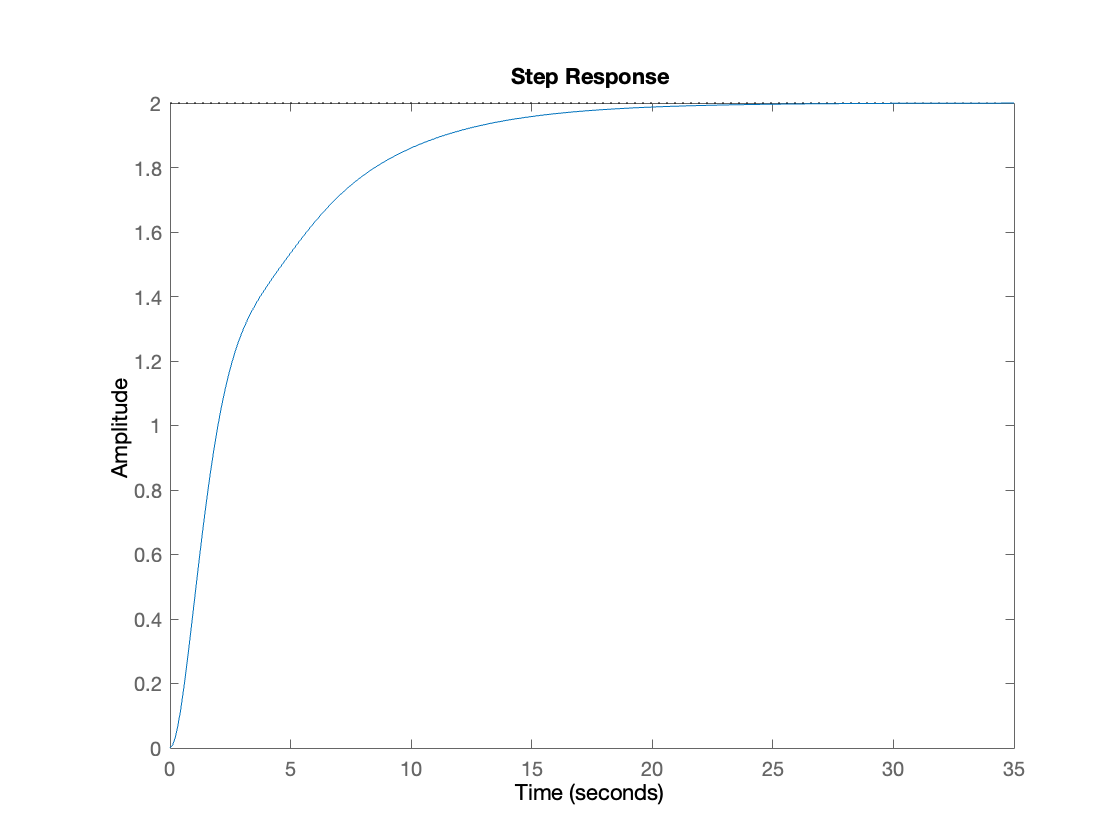
\includegraphics[width=0.7\linewidth]{./figures/step_response.png}
%     \caption{Step Response}
%     \label{fig:step}
%  \end{figure}



\end{document}

